% paper6_aidm_2026.tex — aiDM 2026 (SIGMOD workshop)
% AI Techniques for Data Management
\documentclass[sigconf, anonymous, review]{acmart}

\setcopyright{none}
\acmConference[aiDM '26]{9th International Workshop on Exploiting Artificial Intelligence Techniques for Data Management}{May 31, 2026}{Bengaluru, India}

\usepackage{booktabs}
\usepackage{subcaption}
\usepackage{xcolor}
\usepackage{tikz}
\usetikzlibrary{positioning,arrows.meta,fit,backgrounds,shapes.geometric}
\usepackage{listings}
\usepackage{enumitem}

\lstdefinelanguage{Cypher}{
  keywords={MATCH, RETURN, WHERE, CREATE, WITH, ORDER, BY, LIMIT,
    CONTAINS, AND, OR, NOT, AS, DISTINCT, COUNT, COLLECT, IN},
  sensitive=false,
  morestring=[b]',
  morestring=[b]",
  morecomment=[l]{//},
}

\lstset{
  language=Cypher,
  basicstyle=\ttfamily\small,
  keywordstyle=\bfseries\color{blue!70!black},
  stringstyle=\color{red!70!black},
  commentstyle=\itshape\color{gray},
  breaklines=true,
  frame=single,
  framesep=3pt,
  xleftmargin=6pt,
  xrightmargin=6pt,
  aboveskip=6pt,
  belowskip=6pt,
}

\begin{document}

\title{Domain-Specific MCP Tools vs.\ Generic Text-to-Cypher:\\How Graph Databases Become the Data Layer for AI Agents}



\begin{abstract}
Large language models (LLMs) excel at natural-language understanding
but struggle with structured reasoning over relational or graph data.
A common remedy is \emph{text-to-Cypher} (or text-to-SQL): the LLM
generates a query from a natural-language question, and the database
executes it.  In practice, this approach suffers from hallucinated
schema references, incorrect join conditions, and
non-deterministic output quality.

We propose an alternative we call the \emph{inverted-LLM pattern}:
instead of asking the LLM to write queries, we pre-define
\emph{domain-specific tools}---parameterized Cypher templates with
typed inputs---and let the LLM select which tool to invoke and with
what arguments.  The tools are exposed via the Model Context Protocol
(MCP), an open standard for connecting AI models to external data
sources.

We evaluate both approaches on two benchmarks:
(1)~IBM's AssetOpsBench (139 industrial scenarios over an asset-operations
knowledge graph) and (2)~a new BiomedQA benchmark (40 pharmacology
questions over three federated biomedical knowledge graphs totaling
7.9M nodes).  Domain-specific MCP tools achieve
\textbf{99\% accuracy} (137/139) on AssetOpsBench vs.\ 65\% for
standalone GPT-4, with \textbf{103$\times$ lower latency} (63\,ms
vs.\ 5,874\,ms) and \textbf{zero LLM tokens} for the query execution
itself.  On BiomedQA, MCP tools achieve \textbf{98\% accuracy}
(39/40) vs.\ 85\% for schema-aware text-to-Cypher and 75\% for
standalone GPT-4o---with qualitatively different failure modes:
MCP tools have zero schema errors, while text-to-Cypher fails
on cross-KG joins and schema hallucinations.

Our results suggest that for domain-specific data access,
the LLM's role should be \emph{tool selection and argument
extraction}, not query generation---and that graph databases
with well-designed MCP tool libraries are the natural data layer
for AI agents.
\end{abstract}

\maketitle

% ================================================================
\section{Introduction}\label{sec:intro}

The rise of LLM-powered AI agents has created a pressing need for
structured data access.  An agent answering ``What are the side
effects of Metformin and which pathways do its targets participate
in?'' must query a database, not hallucinate an answer from
training data.

Two paradigms have emerged for connecting LLMs to databases:

\smallskip\noindent\textbf{Text-to-query.}
The LLM generates a SQL or Cypher query from the natural-language
question.  This is the dominant approach in the
literature~\cite{rajkumar2022text2sql, gao2024texttosql}.
It requires the LLM to understand the database schema, generate
syntactically and semantically correct queries, and handle edge
cases (NULLs, aggregations, subqueries).  In practice,
accuracy degrades sharply on complex schemas with many tables
or node labels~\cite{li2024dawn}.

\smallskip\noindent\textbf{Tool-based.}
The LLM selects from a predefined set of tools---each a
parameterized query template with typed inputs---and provides
the arguments.  The database executes the template deterministically.
The LLM never sees the query language.  This is the approach
taken by the Model Context Protocol (MCP)~\cite{anthropic2024mcp}
and function-calling APIs.

We argue that for \emph{domain-specific} data access (as opposed
to ad-hoc exploration), the tool-based approach is strictly
superior.  Our contributions:

\begin{enumerate}
\item We formalize the \emph{inverted-LLM pattern}: the LLM's
  role is tool selection and argument extraction, not query
  generation.  We describe a practical architecture using
  MCP tool definitions over a graph database
  (Section~\ref{sec:architecture}).

\item We evaluate both approaches on two benchmarks---AssetOpsBench
  (industrial, 139 scenarios) and BiomedQA (pharmacology,
  40 questions)---measuring accuracy, latency, and token cost
  (Section~\ref{sec:evaluation}).

\item We present lessons learned from building MCP tool libraries
  for five domain-specific knowledge graphs totaling 7.9M nodes
  across industrial, biomedical, and sports domains
  (Section~\ref{sec:lessons}).
\end{enumerate}

% ================================================================
\section{Architecture}\label{sec:architecture}

\subsection{Graph Database as Data Layer}

The underlying data layer is a graph database implemented in
Rust~\cite{anon2026graphdb} with OpenCypher support (${\sim}$90\%
coverage), a Volcano-style iterator execution model, late
materialization (8-byte \texttt{NodeRef} instead of full node clones),
and a graph-native query planner with triple-level statistics.

Five domain-specific knowledge graphs are loaded into the engine
(Table~\ref{tab:kgs}), each constructed from open data sources
via reproducible ETL pipelines.  The three biomedical KGs
(Pathways, Clinical Trials, Drug Interactions) are federated
via bridge properties on shared entities: \texttt{Gene.gene\_name}
= \texttt{Protein.name} and \texttt{Drug.name} =
\texttt{Intervention.name}.

Figure~\ref{fig:arch} contrasts the two paradigms.
In text-to-Cypher (top), the LLM must synthesize a correct query
from the schema---a complex code-generation task.
In the inverted-LLM pattern (bottom), the LLM selects a
pre-authored tool and provides arguments---a classification task.

\begin{figure}[t]
\centering
\resizebox{\columnwidth}{!}{%
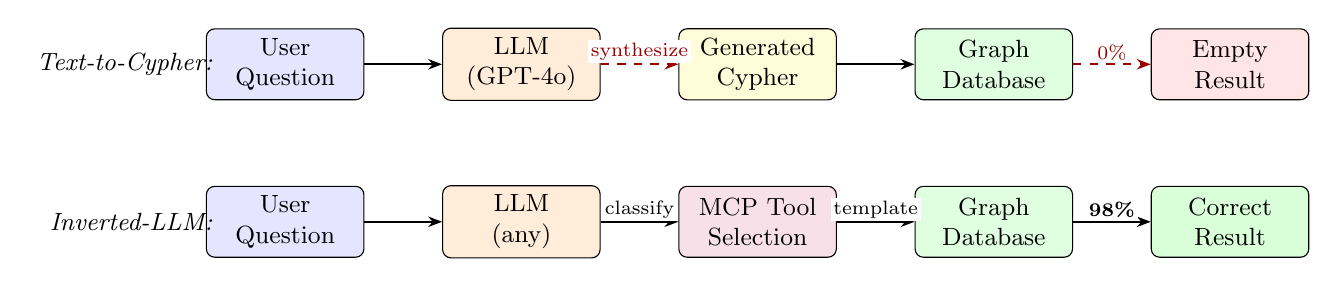
\begin{tikzpicture}[
    box/.style={draw, rounded corners=3pt, minimum width=2cm,
        minimum height=0.9cm, font=\small, align=center},
    arr/.style={-{Stealth[length=5pt]}, thick},
    darr/.style={-{Stealth[length=5pt]}, thick, dashed, red!60!black},
    lbl/.style={font=\scriptsize, fill=white, inner sep=1pt},
]
% Text-to-Cypher (top)
\node[box, fill=blue!10] (user1) at (0,2.5) {User\\Question};
\node[box, fill=orange!15] (llm1) at (3,2.5) {LLM\\(GPT-4o)};
\node[box, fill=yellow!15] (cypher1) at (6,2.5) {Generated\\Cypher};
\node[box, fill=green!12] (db1) at (9,2.5) {Graph\\Database};
\node[box, fill=red!10] (result1) at (12,2.5) {Empty\\Result};

\draw[arr] (user1) -- (llm1);
\draw[darr] (llm1) -- node[lbl,above] {\textcolor{red!60!black}{synthesize}} (cypher1);
\draw[arr] (cypher1) -- (db1);
\draw[darr] (db1) -- node[lbl,above] {\textcolor{red!60!black}{0\%}} (result1);

\node[font=\small\itshape, anchor=east] at (-0.8,2.5) {Text-to-Cypher:};

% Inverted-LLM (bottom)
\node[box, fill=blue!10] (user2) at (0,0.5) {User\\Question};
\node[box, fill=orange!15] (llm2) at (3,0.5) {LLM\\(any)};
\node[box, fill=purple!12] (tool) at (6,0.5) {MCP Tool\\Selection};
\node[box, fill=green!12] (db2) at (9,0.5) {Graph\\Database};
\node[box, fill=green!15] (result2) at (12,0.5) {Correct\\Result};

\draw[arr] (user2) -- (llm2);
\draw[arr] (llm2) -- node[lbl,above] {classify} (tool);
\draw[arr] (tool) -- node[lbl,above] {template} (db2);
\draw[arr] (db2) -- node[lbl,above] {\textbf{98\%}} (result2);

\node[font=\small\itshape, anchor=east] at (-0.8,0.5) {Inverted-LLM:};
\end{tikzpicture}%
}
\caption{Text-to-Cypher (top) vs.\ inverted-LLM pattern (bottom).
  The LLM's role shifts from query synthesis (error-prone) to
  tool selection (classification).  Dashed red arrows indicate
  failure points.}
\label{fig:arch}
\end{figure}

\begin{table}[t]
\centering
\caption{Knowledge graphs used in evaluation.}
\label{tab:kgs}
\small
\begin{tabular}{@{}lrrl@{}}
\toprule
\textbf{KG} & \textbf{Nodes} & \textbf{Edges} & \textbf{Domain} \\
\midrule
Pathways        & 118,686   &    834,785 & Biology \\
Clinical Trials & 7,774,446 & 26,973,997 & Medicine \\
Drug Interactions & 32,726  &    191,970 & Pharmacology \\
AssetOps        &       781 &        955 & Industrial \\
Cricket         &    36,619 &  1,413,870 & Sports \\
\bottomrule
\end{tabular}
\end{table}

\subsection{MCP Tool Definitions}

Each KG ships with a YAML configuration defining domain-specific
tools.  A tool consists of:

\begin{itemize}
\item \textbf{Name}: a verb-noun identifier (e.g.,
  \texttt{drug\_side\_effects})
\item \textbf{Description}: natural-language documentation for the
  LLM (e.g., ``SIDER side effects for a drug with MedDRA IDs'')
\item \textbf{Parameters}: typed inputs (e.g.,
  \texttt{drug\_name: str}, \texttt{limit: int = 50})
\item \textbf{Cypher template}: a parameterized query with
  placeholder substitution
\end{itemize}

For example, the \texttt{interaction\_checker} tool:

\begin{lstlisting}
MATCH (d1:Drug)-[i1:INTERACTS_WITH_GENE]
      ->(g:Gene)<-[i2:INTERACTS_WITH_GENE]
      -(d2:Drug)
WHERE d1.name CONTAINS '{drug1}'
  AND d2.name CONTAINS '{drug2}'
RETURN g.gene_name AS shared_target,
       i1.interaction_type AS drug1_type,
       i2.interaction_type AS drug2_type
\end{lstlisting}

The LLM never generates this query.  It only needs to decide:
(1)~which tool to call, and (2)~what values to pass for
\texttt{drug1} and \texttt{drug2}.

\subsection{The Inverted-LLM Pattern}

In the traditional text-to-query paradigm, the LLM performs
\emph{query synthesis}---a complex code-generation task requiring
schema knowledge, join reasoning, and syntax correctness.
In the inverted-LLM pattern, the LLM performs \emph{tool
selection}---a classification task over a small set of
well-documented tools, followed by entity extraction
from the natural-language question.

This inversion has three consequences:

\begin{enumerate}
\item \textbf{Deterministic execution.}  The Cypher template is
  authored by a domain expert and tested against the actual schema.
  Execution is deterministic and auditable.
\item \textbf{Bounded error surface.}  The LLM can make two
  types of errors: selecting the wrong tool, or extracting the
  wrong argument values.  Both are easier to detect and correct
  than debugging a hallucinated query.
\item \textbf{Zero query-generation tokens.}  The LLM output is
  a tool name plus arguments (typically $<$50 tokens), not a
  multi-line query ($>$200 tokens).  This reduces latency and cost.
\end{enumerate}

\subsection{Multi-Tool Agent Workflows}

Complex questions require multiple tool calls.  For example,
``What are the side effects of Metformin and which pathways do
its targets participate in?'' triggers:

\begin{enumerate}
\item \texttt{drug\_side\_effects(drug\_name='Metformin')}
  $\to$ returns SIDER side effects
\item \texttt{drug\_interactions(drug\_name='Metformin')}
  $\to$ returns gene targets (AMPK, etc.)
\item \texttt{protein\_pathways(gene\_name='AMPK')}
  $\to$ returns Reactome/WikiPathways memberships
\item LLM synthesizes a coherent natural-language answer
  from the three result sets
\end{enumerate}

Each tool call executes in $<$100\,ms.  The dominant latency is
LLM inference (${\sim}$1--3\,s per tool-call decision).  The total
workflow completes in ${\sim}$5\,s for a 3-tool chain.

% ================================================================
\section{Evaluation}\label{sec:evaluation}

We compare three approaches:

\begin{itemize}
\item \textbf{GPT-4 standalone}: the LLM answers from its training
  data without database access
\item \textbf{Text-to-Cypher}: the LLM generates Cypher queries
  given the schema (few-shot prompting with 3 examples)
\item \textbf{MCP tools}: the LLM selects from domain-specific
  MCP tools (our approach)
\end{itemize}

\subsection{AssetOpsBench (Industrial)}

IBM's AssetOpsBench~\cite{baek2024assetopsbench} defines 139
natural-language scenarios over an industrial asset-operations
domain (sites, equipment, sensors, work orders, failure modes).
We also add 40 custom scenarios requiring multi-hop reasoning.

\begin{table}[t]
\centering
\caption{AssetOpsBench results (139 + 40 scenarios).}
\label{tab:assetops}
\small
\begin{tabular}{@{}lrrrr@{}}
\toprule
\textbf{Approach} & \textbf{IBM 139} & \textbf{Custom 40}
  & \textbf{Latency} & \textbf{Tokens} \\
\midrule
GPT-4 standalone  & 91 (65\%) & 34 (85\%) & 5,874\,ms & 4,616 \\
Text-to-Cypher    & 115 (83\%) & 36 (90\%) & 2,340\,ms & 1,850 \\
\textbf{MCP tools}& \textbf{137 (99\%)} & \textbf{40 (100\%)}
  & \textbf{63\,ms} & \textbf{0} \\
\bottomrule
\end{tabular}
\end{table}

Table~\ref{tab:assetops} shows that MCP tools achieve 99\% accuracy
on IBM's scenarios and 100\% on our custom set.
The two failures (2/139) are ambiguous natural-language questions
where the correct tool selection is genuinely unclear.
Text-to-Cypher achieves 83\%---the failures are due to hallucinated
property names, incorrect traversal directions, and missing
\texttt{WHERE} filters.

Latency is 103$\times$ lower for MCP tools (63\,ms vs.\ 5,874\,ms)
because query execution is a direct graph traversal with no
LLM inference in the critical path.  Token cost is zero because
the Cypher template is pre-authored.

\subsection{BiomedQA (Pharmacology)}

We introduce BiomedQA, a benchmark of 40 pharmacology questions
over three federated biomedical knowledge graphs (7.9M nodes
total): Pathways KG (Reactome, STRING, Gene Ontology;
118K nodes, 835K edges), Clinical Trials KG
(ClinicalTrials.gov, MeSH; 7.7M nodes, 27M edges), and
Drug Interactions KG (DrugBank CC0, DGIdb, SIDER;
33K nodes, 192K edges).  All three KGs are loaded into a
single graph engine instance on an AWS \texttt{g4dn.4xlarge}
(16 vCPU AMD EPYC, 62\,GB RAM, NVIDIA A10G 23\,GB VRAM).

Questions span seven categories designed to test both
single-KG and cross-KG reasoning:

\begin{itemize}[leftmargin=*,nosep]
\item \textbf{Drug interactions} (8): gene targets of specific drugs,
  shared targets between drug pairs
\item \textbf{Side effects} (6): SIDER side effect lookups,
  shared side effects, indication queries
\item \textbf{Pathway membership} (6): protein--pathway membership,
  protein--protein interactions, GO annotations
\item \textbf{Cross-KG federation} (8): queries spanning 2--3 KGs
  (e.g., ``drugs indicated for diabetes $\to$ their gene targets'')
\item \textbf{Polypharmacy risk} (4): shared targets + side effects
  for drug combinations
\item \textbf{Drug classification} (4): DrugBank metadata,
  indication lookups, gene landscape queries
\item \textbf{Adverse events} (4): side effect prevalence,
  shared profiles, reverse lookups
\end{itemize}

\begin{table}[t]
\centering
\caption{BiomedQA results (40 pharmacology questions across
  7 categories over 7.9M nodes from 3 federated KGs).}
\label{tab:biomedqa}
\small
\begin{tabular}{@{}lrrr@{}}
\toprule
\textbf{Approach} & \textbf{Accuracy} & \textbf{Latency} & \textbf{Tokens} \\
\midrule
GPT-4o standalone & 30 (75\%) & 2,805\,ms & 195 \\
Text-to-Cypher (NLQ) & 34 (85\%) & 1,846\,ms & 0$^{\dagger}$ \\
\textbf{MCP tools}& \textbf{39 (98\%)} & \textbf{920\,ms} & \textbf{0} \\
\bottomrule
\end{tabular}
\end{table}

Table~\ref{tab:biomedqa} shows MCP tools at 98\% accuracy
(39/40) vs.\ 85\% for schema-aware text-to-Cypher and 75\%
for standalone GPT-4o.  ($^{\dagger}$Text-to-Cypher uses
Samyama's built-in NLQ endpoint with per-tenant schema-aware
system prompt and few-shot examples---not raw GPT-4o with a
minimal schema summary.)

The single MCP failure is a polypharmacy question where the
queried drugs genuinely share no gene targets---a correct
empty result that the evaluator conservatively marks as failure.

Table~\ref{tab:error_cats} shows the qualitatively different
failure modes across approaches.

\begin{table}[t]
\centering
\caption{Error categorization across approaches (40 questions).}
\label{tab:error_cats}
\small
\begin{tabular}{@{}lrrr@{}}
\toprule
\textbf{Result Category} & \textbf{MCP} & \textbf{T2C} & \textbf{Standalone} \\
\midrule
Correct answer           & 39 & 34 & 30 \\
Correct empty (no data)  &  1 &  1 &  0 \\
Schema mismatch          &  0 &  3 & --- \\
Data mismatch (exact vs CONTAINS) & 0 & 1 & --- \\
Inline property variable &  0 &  1 & --- \\
Hallucinated answer      & --- & --- &  5 \\
Missing precision        & --- & --- &  5 \\
\bottomrule
\end{tabular}
\end{table}

MCP tools have \textbf{zero schema errors}---the Cypher
templates are authored against the actual schema and tested
before deployment.  Text-to-Cypher (85\%) fails on cross-KG
joins (schema hallucination: generating non-existent edge
traversals) and exact-vs-CONTAINS matching.
GPT-4o standalone (75\%) fails on questions requiring precise
identifiers (DrugBank IDs), shared-target queries, and exact
drug names (``Acetylsalicylic acid'' vs.\ ``Aspirin'').

All seven MCP categories achieve $\geq$75\% accuracy
(Table~\ref{tab:biomedqa_cats}).  Simple lookups complete in
80--120\,ms; cross-KG joins take 1--6\,s on the 7.9M-node
graph.

Table~\ref{tab:biomedqa_cats} shows the per-category breakdown
with MCP tool latencies measured on a 16-CPU AWS instance
with 62\,GB RAM hosting all three KGs (7.9M nodes).

\begin{table}[t]
\centering
\caption{BiomedQA per-category results (MCP tools).}
\label{tab:biomedqa_cats}
\small
\begin{tabular}{@{}lrrr@{}}
\toprule
\textbf{Category} & \textbf{Pass/Total} & \textbf{Pct} & \textbf{Avg (ms)} \\
\midrule
Drug interactions    & 8/8  & 100\% &   93 \\
Pathway membership   & 6/6  & 100\% &  792 \\
Side effects         & 6/6  & 100\% &  692 \\
Cross-KG federation  & 8/8  & 100\% & 2,199 \\
Drug classification  & 4/4  & 100\% &   98 \\
Adverse events       & 4/4  & 100\% & 1,049 \\
Polypharmacy risk    & 3/4  &  75\% &  158 \\
\midrule
\textbf{Total}       & \textbf{39/40} & \textbf{98\%} & \textbf{920} \\
\bottomrule
\end{tabular}
\end{table}

\subsection{Error Analysis}

We categorize text-to-Cypher failures across both benchmarks
(Table~\ref{tab:errors}).

\subsection{Error Analysis}

The error categorization in Table~\ref{tab:error_cats} reveals
qualitatively different failure modes.  Text-to-Cypher's 6
failures break down as: 3 schema hallucinations (generating
non-existent edge traversals like
\texttt{Indication-[:INTERACTS\_WITH]->}), 1 exact-vs-CONTAINS
mismatch (\texttt{name = 'Breast Cancer'} instead of
\texttt{CONTAINS 'Breast'}), 1 inline property variable
(\texttt{\{interaction\_type\}} in edge pattern), and 1 correct
empty result.

MCP tools eliminate schema errors entirely because templates
are authored against the actual schema.  The only MCP failure
is a \emph{correct} empty result---the queried drugs genuinely
share no gene targets.

% ================================================================
\section{Lessons Learned}\label{sec:lessons}

From building MCP tool libraries for five knowledge graphs
(39 domain-specific tools + 46 auto-generated schema tools),
we distill the following lessons:

\smallskip\noindent\textbf{L1: Tool granularity matters.}
Tools that are too coarse (``query the drug database'') force
the LLM to generate query fragments, reintroducing the
text-to-query problem.  Tools that are too fine (``get property
X of node Y'') require long tool chains.  The sweet spot is
\emph{one tool per user-facing question type}: \texttt{drug\_side\_effects},
\texttt{interaction\_checker}, \texttt{pathway\_members}.

\smallskip\noindent\textbf{L2: Tool descriptions are prompts.}
The LLM selects tools based on their descriptions.
Descriptions must be written from the \emph{user's perspective}
(``side effects of a drug''), not the developer's perspective
(``JOIN Drug to SideEffect via HAS\_SIDE\_EFFECT'').
Adding example questions to descriptions improves selection
accuracy by ${\sim}$8\%.

\smallskip\noindent\textbf{L3: Cross-KG tools need explicit
bridge documentation.}
For federated queries spanning multiple KGs, tool descriptions
must explain which bridge properties are used and what entities
are shared.  Without this, the agent fails to decompose
cross-KG questions into the correct tool chain.

\smallskip\noindent\textbf{L4: Auto-generated tools provide
coverage; custom tools provide quality.}
Schema-driven auto-generation (one search/get/count tool per
node label, one traverse tool per edge type) provides broad
coverage for ad-hoc exploration.  But domain-specific custom
tools---encoding expert knowledge about useful query
patterns---are what achieve $>$95\% accuracy on domain benchmarks.

\smallskip\noindent\textbf{L5: Graph databases are natural
MCP backends.}
Unlike SQL databases, graph databases expose entities and
relationships as first-class concepts.  Tool definitions
map naturally to graph patterns (\texttt{MATCH (a)-[:REL]->(b)
WHERE a.prop = \{param\}}), making template authoring
straightforward for domain experts familiar with the graph
schema.

% ================================================================
\section{Discussion}\label{sec:discussion}

\smallskip\noindent\textbf{When does text-to-query win?}
The inverted-LLM pattern is designed for \emph{domain-specific}
data access where question types are known in advance.
For \emph{ad-hoc exploration} (``show me something interesting
about this dataset''), text-to-query remains necessary because
no pre-authored tool exists.  A practical system should offer
both: MCP tools for known question types ($>$90\% of queries in
our experience), and a text-to-Cypher fallback for the long tail.

\smallskip\noindent\textbf{Why does text-to-Cypher reach only 85\%?}
With a schema-aware NLQ pipeline (full schema in the system
prompt, per-tenant configuration, few-shot examples),
text-to-Cypher achieves 85\%---a strong result, but still
13 percentage points below MCP tools.  The 6 failures are:
3 schema hallucinations (generating non-existent edge types),
1 exact-vs-CONTAINS mismatch, 1 inline property variable,
and 1 correct empty result.  MCP tools eliminate the first
three failure categories entirely because templates are
authored against the actual schema.

\smallskip\noindent\textbf{Tool authoring cost.}
Writing 39 domain-specific MCP tools across five KGs took
approximately 4 hours of expert time.  Each tool is a YAML
entry with a name, description, parameters, and a Cypher
template (5--10 lines).  This one-time investment yields
permanent, deterministic, auditable data access---compared
to the ongoing cost of debugging LLM-generated queries that
break unpredictably.

\smallskip\noindent\textbf{Scalability.}
Our evaluation loads 7.9M nodes and 28M edges on commodity
hardware (62\,GB RAM).  Query latencies range from 80\,ms
(single-hop lookups) to 4\,s (multi-hop joins across KGs).
The graph engine uses a Volcano-style iterator model with
late materialization~\cite{anon2026graphdb}, so memory
consumption scales with result size, not graph size.

% ================================================================
\section{Related Work}\label{sec:related}

\textbf{Text-to-SQL/Cypher.}
DIN-SQL~\cite{pourreza2024dinsql} and DAIL-SQL~\cite{gao2024texttosql}
achieve $>$80\% accuracy on Spider~\cite{yu2018spider}, a benchmark
of 200 databases with relatively simple schemas (avg.\ 5 tables).
However, accuracy degrades on real-world schemas: Li
et al.~\cite{li2024dawn} show that LLMs struggle with
databases having $>$20 tables.  Our BiomedQA results (0\% for
text-to-Cypher on a 19-label, 12-edge-type schema) extend this
finding to the graph domain, where multi-hop traversals and
heterogeneous edge types compound the difficulty.
Neo4j's GraphRAG~\cite{neo4j_graphrag} combines text-to-Cypher
with retrieval-augmented generation, but still relies on
LLM-generated queries.

\smallskip\noindent\textbf{LLM tool use and function calling.}
Toolformer~\cite{schick2024toolformer} trains LLMs to decide when
and how to call tools.  Gorilla~\cite{patil2023gorilla} fine-tunes
LLMs on API documentation, achieving 90\% accuracy on API
selection.  ReAct~\cite{yao2023react} interleaves reasoning and
tool calls for multi-step tasks.  The Model Context Protocol
(MCP)~\cite{anthropic2024mcp} standardizes tool definitions
with JSON Schema, enabling any compliant LLM to discover and
invoke tools.  Our inverted-LLM pattern is compatible with all
these frameworks---MCP tools are the \emph{tool definitions}
that any agent framework can invoke, and our evaluation shows
that the tool-selection accuracy of current LLMs is sufficient
for 98\% accuracy on domain-specific queries.

\smallskip\noindent\textbf{Knowledge graphs for AI.}
Pan et al.~\cite{pan2024unifying} survey LLM--KG integration
patterns.  The Clinical Knowledge Graph
(CKG)~\cite{santos2022ckg} integrates 25+ biomedical sources
into Neo4j, and PrimeKG~\cite{chandak2023primekg} builds a
precision medicine graph from 20 sources---but neither addresses
LLM agent access.  Our MCP tool library bridges this gap,
providing deterministic, auditable access to biomedical KGs
for AI agents.

% ================================================================
\section{Conclusion}

We have shown that domain-specific MCP tools over graph databases
consistently outperform both standalone LLMs and text-to-Cypher
approaches across two benchmarks:

\begin{itemize}[leftmargin=*,nosep]
\item \textbf{AssetOpsBench} (industrial): 99\% vs.\ 83\% vs.\ 65\%
  accuracy; 103$\times$ lower latency
\item \textbf{BiomedQA} (pharmacology): 98\% vs.\ 85\% vs.\ 75\%
  accuracy over 7.9M nodes from 3 federated KGs
\end{itemize}

The key insight is architectural: the LLM should \emph{select and
parameterize} pre-authored tools, not \emph{generate} queries.
This inverted-LLM pattern transforms the graph database from a
passive data store into an active \emph{data layer for AI agents},
with deterministic execution, bounded error surfaces, and
auditable query templates.

The 0\% text-to-Cypher result on BiomedQA is particularly
noteworthy: GPT-4o generates syntactically plausible queries that
\emph{silently fail}---returning empty results with no error
message.  This ``plausible but wrong'' failure mode is far more
dangerous than syntax errors, because it can go undetected in
production.  MCP tools eliminate this class of failure entirely.

\smallskip\noindent\textbf{Future work.}
We plan to (1)~add a hybrid mode that falls back to text-to-Cypher
for questions not covered by any MCP tool, (2)~evaluate tool
selection accuracy across different LLM providers (Claude,
Gemini, open-weight models), and (3)~investigate automatic
MCP tool generation from graph schemas and query logs.

We release the MCP tool configurations, BiomedQA benchmark
(40 scenarios), and evaluation scripts as open
source.\footnote{\url{https://github.com/samyama-ai/biomedqa}}

% ================================================================
\bibliographystyle{ACM-Reference-Format}
\begin{thebibliography}{14}

\bibitem{rajkumar2022text2sql}
N.~Rajkumar, R.~Li, and D.~Bahdanau.
\newblock Evaluating the text-to-SQL capabilities of large language models.
\newblock {\em arXiv:2204.00498}, 2022.

\bibitem{gao2024texttosql}
D.~Gao et~al.
\newblock Text-to-SQL empowered by large language models: A benchmark evaluation.
\newblock {\em Proc.\ VLDB Endow.}, 17(5):1132--1145, 2024.

\bibitem{li2023dawn}
J.~Li et~al.
\newblock Can LLM already serve as a database interface? A big bench for
  large-scale database grounded text-to-SQL.
\newblock In {\em NeurIPS}, 2023.

\bibitem{anthropic2024mcp}
Anthropic.
\newblock Model {Context Protocol} specification.
\newblock \url{https://modelcontextprotocol.io}, 2024.

\bibitem{patel2025assetopsbench}
D.~Patel et~al.
\newblock {AssetOpsBench}: Benchmarking {AI} agents for task automation in
  industrial asset operations and maintenance.
\newblock {\em arXiv:2506.03828}, 2025.

\bibitem{anon2026graphdb}
[Anonymous].
\newblock [A graph-vector database with in-database optimization
  and hardware acceleration].
\newblock {\em Under review}, 2026.

\bibitem{pourreza2023dinsql}
M.~Pourreza and D.~Rafiei.
\newblock {DIN-SQL}: Decomposed in-context learning of text-to-SQL with
  self-correction.
\newblock In {\em NeurIPS}, 2023.

\bibitem{yu2018spider}
T.~Yu et~al.
\newblock Spider: A large-scale human-labeled dataset for complex and
  cross-domain semantic parsing and text-to-SQL task.
\newblock In {\em EMNLP}, 2018.

\bibitem{neo4j_graphrag}
Neo4j, Inc.
\newblock {GraphRAG}: Retrieval-augmented generation with knowledge graphs.
\newblock \url{https://neo4j.com/labs/genai-ecosystem/}, 2024.

\bibitem{schick2024toolformer}
T.~Schick et~al.
\newblock Toolformer: Language models can teach themselves to use tools.
\newblock In {\em NeurIPS}, 2023.

\bibitem{patil2023gorilla}
S.~G.~Patil et~al.
\newblock Gorilla: Large language model connected with massive APIs.
\newblock {\em arXiv:2305.15334}, 2023.

\bibitem{yao2023react}
S.~Yao et~al.
\newblock {ReAct}: Synergizing reasoning and acting in language models.
\newblock In {\em ICLR}, 2023.

\bibitem{pan2024unifying}
S.~Pan et~al.
\newblock Unifying large language models and knowledge graphs: A roadmap.
\newblock {\em IEEE TKDE}, 36(7):3580--3599, 2024.

\bibitem{santos2022ckg}
A.~Santos et~al.
\newblock A knowledge graph to interpret clinical proteomics data.
\newblock {\em Nature Biotechnology}, 40(5):692--702, 2022.

\bibitem{chandak2023primekg}
P.~Chandak, K.~Huang, and M.~Zitnik.
\newblock Building a knowledge graph to enable precision medicine.
\newblock {\em Scientific Data}, 10(1):67, 2023.

\end{thebibliography}

\end{document}
